\begin{figure*}[htbp] 
\centering 
 
	\subfigure[\textit{F}-DEA]
	{
		\label{fig:dtlz710fdeafigure}
		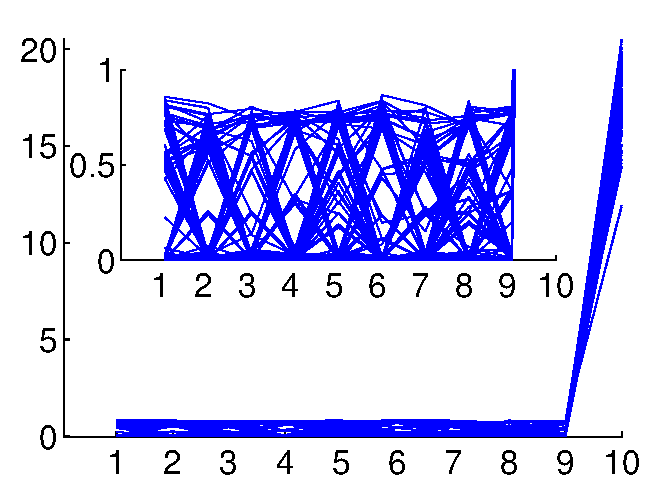
\includegraphics[width=0.170\textwidth]{figures/experiments/dtlz/fdeadtlz7_10.eps}
	}
	\hspace{0em}	
	\subfigure[NSGAIII]
	{
		\label{fig:dtlz710nsgaiiifigure}
		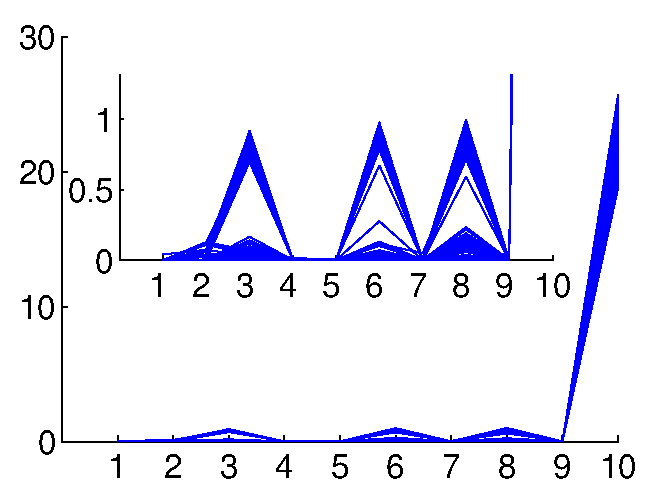
\includegraphics[width=0.170\textwidth]{figures/experiments/dtlz/nsgaiiidtlz7_10.eps}
	}	
	\hspace{0em}
%	\subfigure[MOEA/D]
%	{
%		\label{fig:dtlz710moeadfigure}
%		\includegraphics[width=0.170\textwidth]{figures/experiments/dtlz/moeaddtlz7_10.eps}
%	}	
	\hspace{0em}	
	\subfigure[FD-NSGAII]
	{
		\label{fig:dtlz710zhenanfigure}
		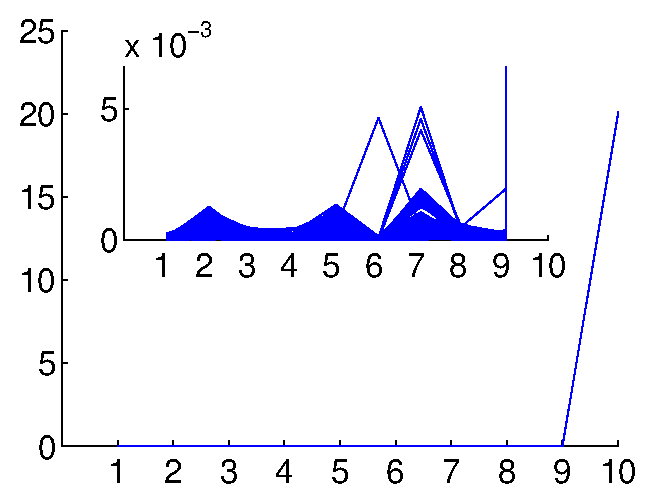
\includegraphics[width=0.170\textwidth]{figures/experiments/dtlz/zhenandtlz7_10.eps}
	}	
%	\hspace{0em}
%	\subfigure[HypE]
%	{
%		\label{fig:dtlz710hypefigure}
%		\includegraphics[width=0.170\textwidth]{figures/experiments/dtlz/hypedtlz7_10.eps}
%	}	
	\hspace{0em}	
	\subfigure[SDE]
	{
		\label{fig:dtlz710sdefigure}
		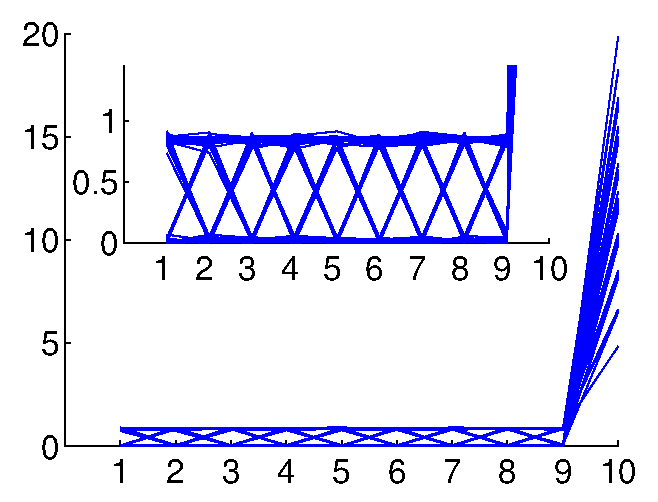
\includegraphics[width=0.170\textwidth]{figures/experiments/dtlz/sdedtlz7_10.eps}
	}	
	\hspace{0em}
	\subfigure[PICEAg]
	{
		\label{fig:dtlz710piceagfigure}
		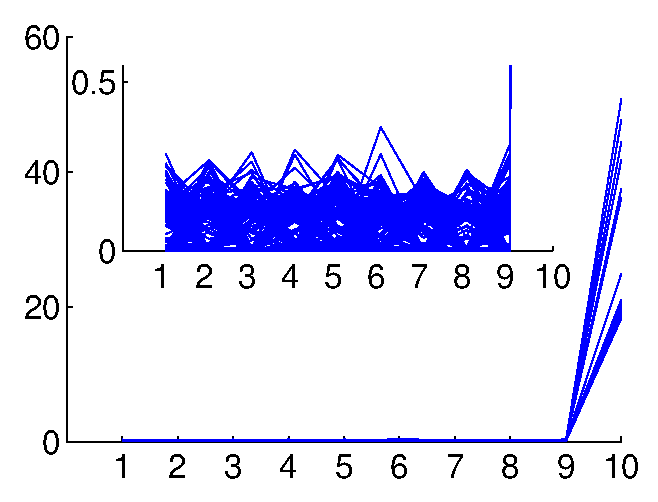
\includegraphics[width=0.170\textwidth]{figures/experiments/dtlz/piceagdtlz7_10.eps}
	}	
\caption{Parallel coordinate plot of all competing algorithms in $10-$ objective DTLZ7 problem. The inset figure shows the closer inspection of the first 9 objectives.}
\label{fig:dtlz710figure}
\end{figure*}